\documentclass[11pt,letterpaper]{article}
%\documentclass[11pt,a4paper]{report}

\usepackage{amssymb,amsmath,amsthm} 
\usepackage[margin=2cm]{geometry}
\usepackage{fancyhdr}
\usepackage{enumitem}
\usepackage[compact]{titlesec}
\usepackage{graphicx,ctable,booktabs,subcaption}

\usepackage{xparse,hyperref,parskip}

%\newcommand{\abs}[1]{\left|#1\right|}

\newcommand{\semester}{Spring 2022}
\newcommand{\due}{Tuesday, April 12}


\pagestyle{fancy}
\lhead{ }
\chead{\footnotesize Math 3338\quad  Numerical Methods\quad  \semester}
\rhead{\footnotesize \thepage}
\setlength{\parindent}{0cm}
\setlist{noitemsep}



\newtheorem{theorem}{Theorem}

\input{defs.tex}

%Defines the problem environment with arguments Points and Solution gap
\input{problem_env.tex}



\begin{document}

\begin{center}
{\huge{\bf  Numerical Methods}} \\[1.5ex]
{\bf Math 3338 -- \semester}\\[1.5ex]
{\Large{\bf Worksheet 23\ \\[2ex] Animations and Chaos}}\\
\end{center}
\vspace{2mm}


\section{Reading}

\begin{table}[!ht]
 \centering
 \begin{tabular}{ll}
   CP &  8.1, 8.2 \\
 NMEP &  Chapter 7
 \end{tabular}
\caption{Sections Covered}
\end{table}

\section{Overview}
Today we're going to understand the double pendulum and learn how to make an animation 
showing it's motion.

\section{Double Pendulum}
A double pendulum is a pendulum on the end of a pendulum. Figure \ref{fig:pendulum} has an example
of a double pendulum.
\begin{figure}[!ht]
 \centering
 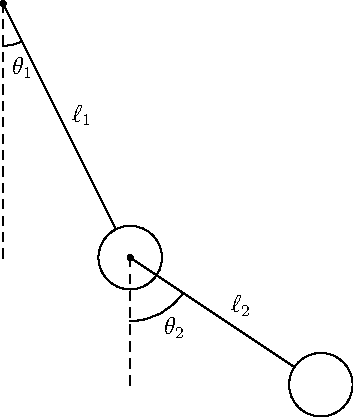
\includegraphics{images/pendulum.pdf}
 \caption{Double Pendulum}
 \label{fig:pendulum}
\end{figure}
This is a classic physics problem as the motion of the second pendulum is chaotic. 

The equations to describe the motion are... a bit much. So we won't derive them. Before you
see them, we need some notation. Dot notation is a nice simplification to Leibniz notation.
\begin{align*}
 \frac{dx}{dt} &= \dot{x} & \frac{d^2x}{dt^2} &= \ddot{x}
\end{align*}
Each dot represents of derivative with respect to time.

We are going to assume the lengths of the rods are the same and the masses of the pendulums are
the same.\footnote{If you don't think we should, be my guest to rederive the equations} Here are
the equations.
\begin{gather*}
 2\ddot{\theta}_1 + \ddot{\theta}_2\cos(\theta_1-\theta_2)+\dot{\theta}_2^2\sin(\theta_1-\theta_2)+2\frac{g}{\ell}\sin(\theta_1)=0\\
\ddot{\theta}_2 + \ddot{\theta}_1\cos(\theta_1-\theta_2)-\dot{\theta}^2_1\sin(\theta_1-\theta_2)+\frac{g}{\ell}\sin(\theta_2)=0
\end{gather*}
However these aren't actually what we solve. We actually solve the following,
\begin{gather*}
\dot{\theta}_1 = \omega_1 \\
\dot{\theta}_2 = \omega_2 \\
\dot{\omega}_1 = -\frac{\omega_1^2\sin(2\theta_1-2\theta_2)+2\omega_2^2\sin(\theta_1-\theta_2)+\frac{g}{l}(\sin(\theta_1-2\theta_2)+3\sin(\theta_1))}{3-\cos(2\theta_1-2\theta_2)} \\
\dot{\omega}_2 = \frac{4\omega_1^2\sin(\theta_1-\theta_2)+\omega_2^2\sin(2\theta_1-2\theta_2)+2\frac{g}{l}(\sin(2\theta_1-\theta_2)-\sin(\theta_2))}{3-\cos(2\theta_1-2\theta_2)} 
\end{gather*}


\section{Animation}
The method I'm about to describe requires FFMPEG which is an encoder algorithm. This \emph{should}
be easy to install on a Mac and is possible on a Windows computer. Alternatively, you can use a different
method to create the animation\footnote{This could be as easy as changing the file extension. But
mp4 is generally the ``best''}.

At it's core, an animation is just a sequence of graphs displayed over time. We need to tell
the computer what the first graph is, and the following graphs. There is an example on Canvas
that should help you get started making animations. 




\newpage

\begin{center}
{\huge{\bf  Numerical Methods}} \\[1.5ex]
{\bf Math 3338 -- \semester}\\[1.5ex]
{\Large{\bf Homework 23 (Due: \due)}}\\
\end{center}
\vspace{2mm}

\begin{problem}
 Write a function that solves the double pendulum. Your inputs should be the two initial angles,
the time domain and the number of steps. You should return a tuple $(\theta_1,\theta_2)$. We'll
assume $g=10$ and $\ell=1$.
\end{problem}


\begin{problem}
 Make a graph of $\theta_1$ vs. $t$ and $\theta_2$ vs $t$ on the same axis. The initial conditions
are $\theta_1=\theta_2=\frac{\pi}{2}$. The domain is 
$0\le t\le 50$ with 1,000 steps. Save this graph as a PDF and include in a tex file. Explain what
this graph is saying.
\end{problem}


\begin{problem}
 Make a graphs of the position of each pendulum as time progresses. This will be $y$ vs $x$. The 
domain will be $0\le t\le 50$ with 1,000 steps. Make a different plot for each initial condition.
\begin{enumerate}
 \item $\theta_1 = \theta_2 = \frac{\pi}{2}$
 \item $\theta_1 = \pi$, $\theta_2 = \frac{\pi}{2}$
 \item $\theta_1 = \theta_2 = \pi$
\end{enumerate}
Include these in a PDF and explain what each graph is saying.

Note: One of your curves should be a circle representing the inner pendulum.
\end{problem}


\begin{problem}
 Make an animation of the motion of this system for $1\le t\le 50$, 1,000 steps, and initial conditions
$\theta_1 = \pi$ and $\theta_2=\frac{\pi}{2}$. Your plot should include the following,
\begin{enumerate}
 \item A fixed axes, probably $-2.2\le x,y\le 2.2$.
 \item The pendulums. You can do this with two lines, one from the origin and the other from the
end of the first.
 \item The path the inner pendulum traces as it's tracing it.
 \item The path the outer pendulum traces as it's tracing it.
\end{enumerate}
Call this \textbf{double-1000.mp4}.
\end{problem}


\begin{problem}
 Repeat the previous with 500 steps instead of 1,000.
\end{problem}

\begin{problem}
 If you have the computation time, redo with 5,000 steps. This takes about 5 - 15 minutes on my
laptop.
\end{problem}

\begin{problem}
 The three animations you created describe the exact same system, but they aren't perfectly the same.
Why?
\end{problem}


\end{document}




































